\section{Features}

The UCVM platform offers an API and a set of programs, many of which can be used either in a single processor context or in parallel. This section details the most relevant of these programs, categorized by the broad feature they are intended to support. The discussion will focus largely on how the single processor programs operate. Those features that have additional support for parallel computing will be noted, and any operational differences between the single core and parallel implementations shall be described.

The single-core commands can be run in any system where the platform has been successfully installed. The parallel commands, however, require a system where the standard Message Passing Interface (MPI) library and compilers are available. Single-core commands are useful to most users interested in exploring the properties of the regions covered by the models supported by the platform. On the other hand, advanced users needing to build large-scale (regional) materialized velocity models for earthquake modeling and simulation are the more likely to use the MPI commands. 

%\textcolor{green}{For each utility, we should implicitly answer four questions as a narrative. 1) What problem is this utility trying to solve? 2) How does this utility solve the problem? 3) What information does the user need to provide? 4) What does the utility output? For the input description, rather than providing a configuration file, I would use a table with the relevant parameters to the problem and a description of each (ignoring simple things like output file paths, number of processors, etc).}


% ---------------------------------------------------------------------------------------------
% TEMP FIGURE: Needs to be completed and improved in Illustrator and moved to final PDF dir.
\begin{figure*}[ht!]
	\centering
%	\includegraphics
%		[width=0.75\textwidth]
%		{figures/raw-pdf/covered-areas}
	\fbox{\begin{minipage}{\textwidth}\textcolor{red}{PENDING}\vspace{2in}\end{minipage}}
	\caption{Querying a geographic point for material properties.}
	\label{fig:tiling}
\end{figure*}
% ---------------------------------------------------------------------------------------------


\subsection{Querying Material Properties}

UCVM provides two methods for querying models. The first method is programmatically, directly through the provided C language API. The second is via the command-line program \texttt{ucvm\_query}. Both methods query the underying models in the same manner; the \texttt{ucvm\_query} program is merely a simplified front-end layered upon the API.

The query process begins with the identification of one or more CVMs as the source of material properties. In this respect, the framework distinguishes between geo-technical layers and standard crustal models, allowing the user to make selections for both. As illustrated in Figure \ref{fig:tiling}, the set of standard crustal models is tiled in three dimensions to form a meta-model. The same operation is performed on the GTLs to define a meta-GTL. The interface between the meta-GTL and meta-model is then smoothed using an interpolation function (linear interpolation in the simplest case) along a user-defined interpolation zone parallel to the z-axis. Note that when two or more models overlap in three dimensional space, the model listed first within the tiling order will satisfy requests within that overlapping zone.

Once the models have been tiled in this manner, the API or program accepts one or more input query points from the user. For every point, the framework queries each component model of the two meta models, until either a valid set of velocities and density are returned, or all component models have been queried and the request was unsatisfied. Thus, for points that fall within the interpolation zone, two sets of material properties may be generated - one each for each meta model. These two sets of material properties are then combined using the interpolation function. As the native query interfaces of available CVMs accept query points in a wide array of formats (geographic coordinates versus UTM-11 map coordinates, or depth versus elevation for the vertical component, for example), UCVM may perform a coordinate transformation to convert its input format of decimal (latitude, longitude, depth/elevation) tuples to the local coordinate system of the component model being queried. This is accomplished transparently by utilizing the standard projection library Proj.4 (NOTE: cite Proj.4).

In the case of the API, the result of a successful query is a data-structure containing the velocities $V_{p}$ and $V{s}$, and the density $\rho$ at the point of interest, along with the elevation in meters and $V_{S30}$ of the corresponding point on the free-surface, and an indication of which velocity model within the meta-model ultimately satisfied the request. For those points which fall within the interpolation zone between the meta-GTL and meta-model, the framework additionally identifies the material properties reported by the meta-GTL and meta-model, as well as the component models from which they were extracted. For the \texttt{ucvm\_query} program, this same information is formulated in tabular format and printed to the screen.

This tiling mechanism can be a powerful feature for combining multiple regional velocity models, but a problem arises when velocity models overlap in three-dimensional space. Simply tiling two overlapping models will create a three-dimensional interface that may contain sharp contrasts in either velocities or density. This artifact is undesirable for earthquake simulation applications as it can cause reflections in wavefronts. There are two approaches to remedy this problem. The simplest approach is to define a UCVM patch model to trilinearly interpolate the material properties within arbitrary cuboid geographic region. This patch model may be tiled along with the overlapping traditional velocity models to produce a smoothed meta-model. However, this numerical smoothing approach does not reflect the physical structures of the Earth's surface. The second approach is to utilize UCVM to query all models within the overlap zone individually, and then manually combine the results with a user-defined interpolation function. 


\begin{figure*}[ht!]
	\centering
	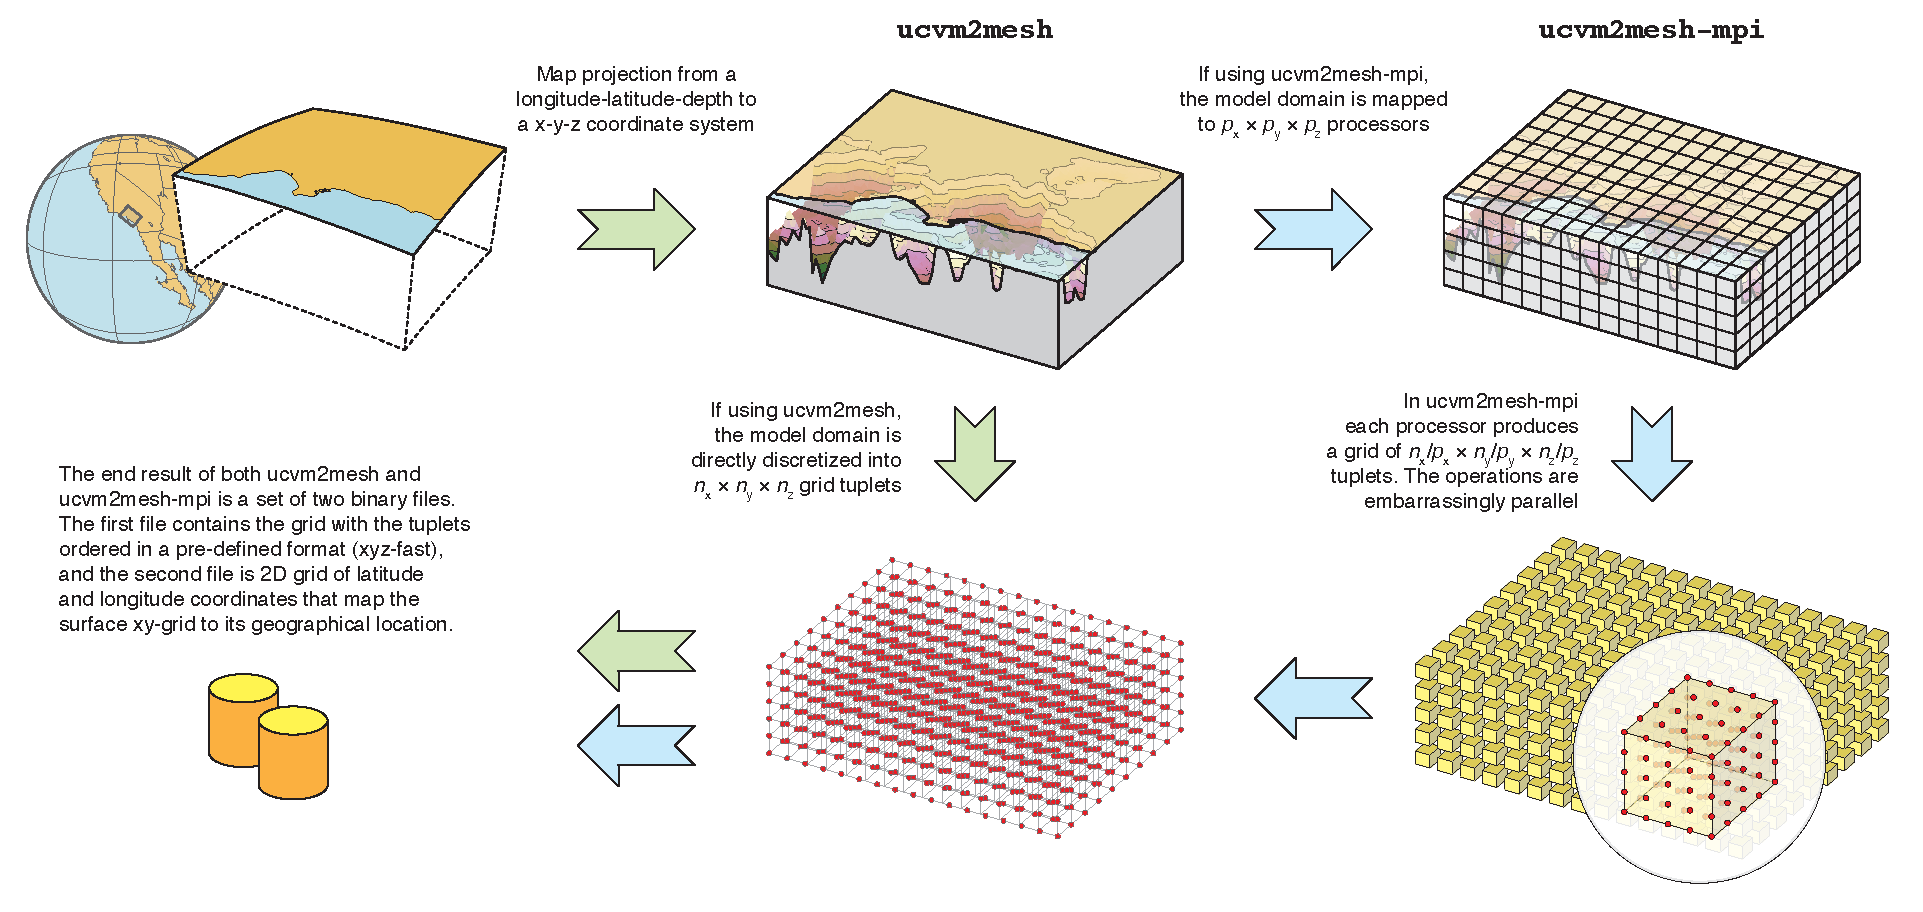
\includegraphics
		[width=\textwidth]
		{figures/pdf/ucvm-to-mesh}
	\caption{Construction of a structured grid with the programs \texttt{ucvm2mesh} (green arrows) and \texttt{ucvm2mesh-mpi} (blue arrows). An important aspect of the gridding process is that the discretized information payload (\vs{}, \vp{}, and $\rho$) is stored at the grid points. That is, the querying and assignment process has a 1-to-1 mapping between the queried point and the grid node of the mesh.}
	\label{fig:meshing}
\end{figure*}


\subsection{Creating Structured 3D Meshes}

The framework may be utilized to generate a structured uniform mesh in a format consistent with those used by the AWP-ODC and SORD (NOTE: need to confirm if SORD still uses this format) simulation codes with the program \texttt{ucvm2mesh}.

Construction of mesh proceeds as shown in Figure \ref{fig:meshing}. The user specifies a two-dimensional map projection (such as UTM-11), a latitude and longitude geographic anchor point, mesh cell dimensions ($nx$, $ny$, $nz$) along the x,y and z axis (where x-y is in the plane of the projection and z is vertical), step size $dx$ in meters, and rotation angle within the map projection. Additionally, the user provides a list of CVMs to query, and these models are tiled in the same manner as was described in the previous section.

The program \texttt{ucvm2mesh} projects the geographic coordinates of the Earth's surface into the map projection, placing the origin of the mesh as the anchor point and discretizing the volume according to the provided dimensions and step size. For each point in the projected volume, \texttt{ucvm2mesh} determines the analous geographic point in terms of (latitude, longitude, depth) and queries the underlying CVMs for material properties. These material properties are then assigned to the mesh point.

Four binary mesh formats are supported: IJK-12, IJK-20, IJK-32, and SORD. The first three formats are mesh variants used by AWP-ODC (NOTE: cite) and the last format is used by SORD (NOTE: cite and check if still true). For IJK-12 formatted meshes, the output is a binary file consisting of a list of nx*ny*nz tuples. Each tuple contains three single precision floating point values $(V_p. V_s, \rho)$, representing the material properties for a point in the mesh, with the mesh coordinates given implicitly by the position of the tuple in the list. The tuples are arranged in x-y-z order. 

Similarly, the IJK-20 format adds the seismological parameters $\mu$ and quality factor $Q$ so that each tuple contains $(V_p. V_s, \rho, mu, Q)$ (NOTE: confirm and explain mu and Q), while the IJK-32 format extends IJK-20 further by adding the three four-byte integers $(i,j,k)$ to each tuple, representing the index coordinate of the grid cell within the mesh. Thus, in this latter case, each tuple contains $(i, j, k, V_p. V_s, \rho, mu, Q)$.

(NOTE: Explain SORD format)

(NOTE: Note ucvm2mesh-mpi exists, I don't think there are any operational differences)


\begin{figure*}[ht!]
	\centering
	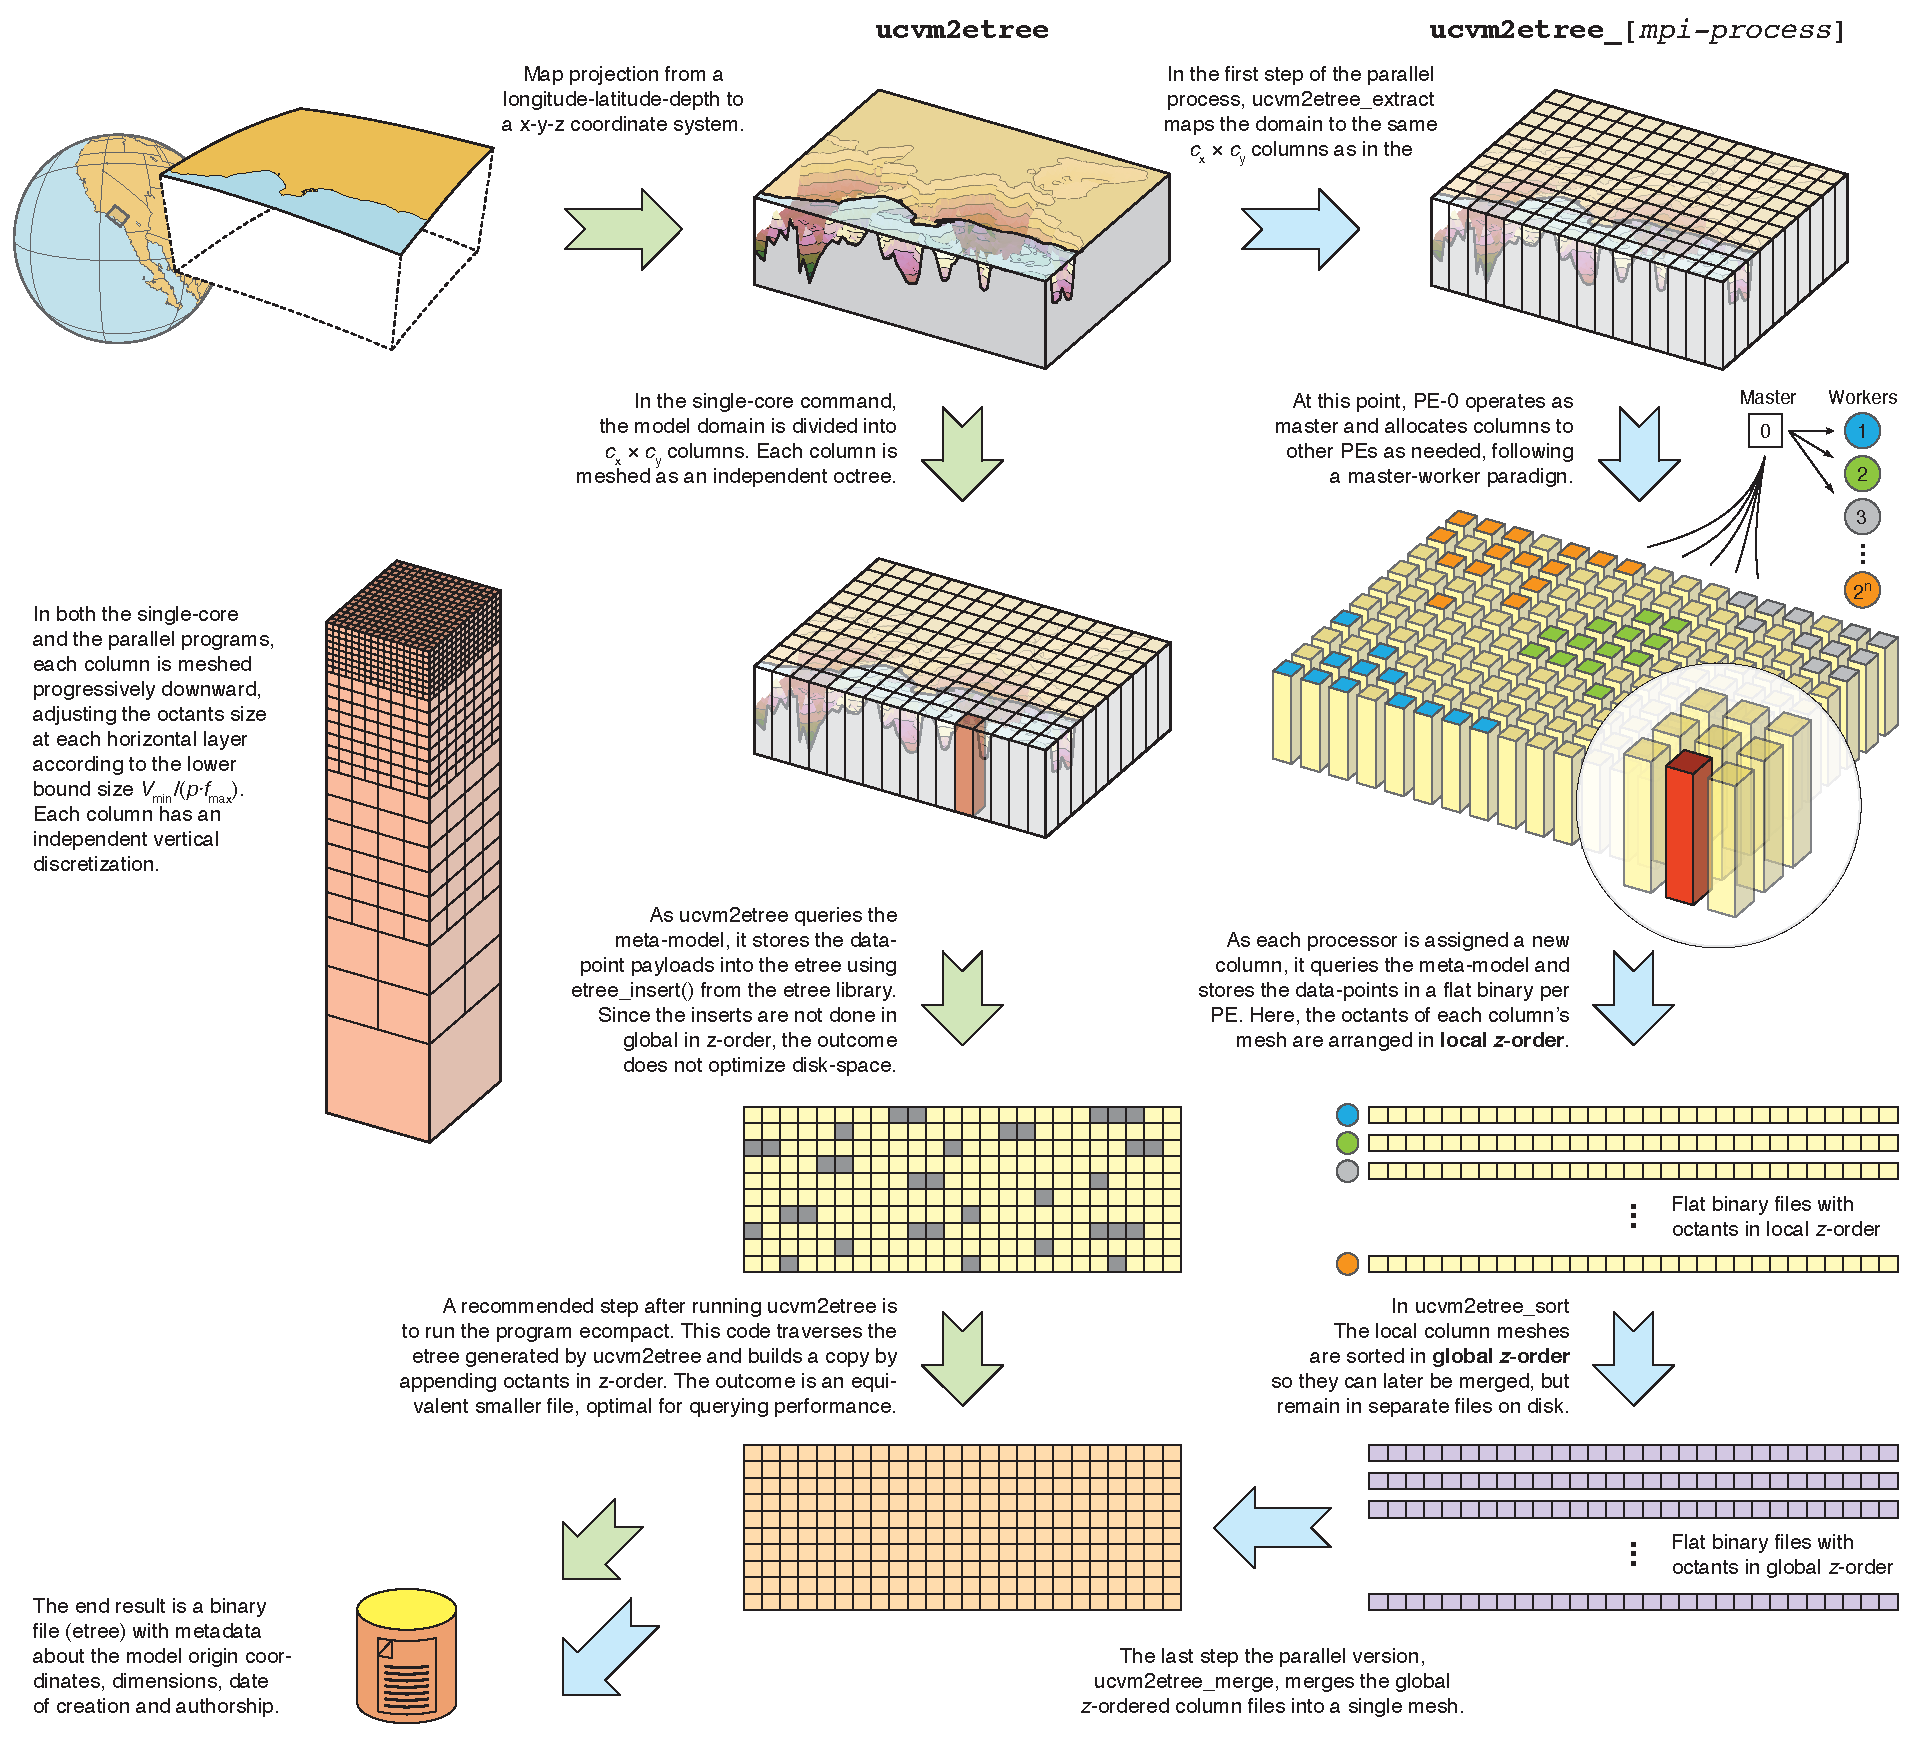
\includegraphics
		[width=\textwidth]
		{figures/pdf/ucvm-to-etree}
	\caption{Construction of an pseudo-unstructured mesh in the Etree database format using the program \texttt{ucvm2etree} and its MPI equivalent processes \texttt{ucvm2etree\_extract}, \texttt{ucvm2etree\_sort} and \texttt{ucvm2etree\_merge}. An important aspect of the meshing-to-etree process is that the discretized information payload (\vs{}, \vp{}, and $\rho$) is stored at the octants in the octree structure. The querying and assignment process mapps the information queried at the center of each octant to the whole volume enclosed by the octant.}
	\label{fig:etrees}
\end{figure*}
% ---------------------------------------------------------------------------------------------


\subsection{Creating Etree Databases}

TBD, reference Figure \ref{fig:etrees}

\subsection{Miscellaneous Features}

TBD

\subsubsection{Querying Iso-surfaces}

TBD 
%\texttt{basin\_query} and \texttt{basin\_query-mpi}


\subsubsection{Small-scale Heterogeneities}

The last decade has seem a tremendous growth on high performance computing and applications dedicated to earthquake ground motion simulations which is leading the charge toward performing deterministic simulations at high frequencies of engineering interest (\fmax{} 0--10 Hz). With increasing simulation frequencies, seismic velocity models must not only be accurate representations of a region's crustal structure at the geologic scale and represent the geotechnical characteristics of basins and deposits, but should also provide for the adequate representation of the scattering characteristics of the typical heterogeneities observed in geomaterials. To this end, UCVM implements an algorithm generates models that incorporate small-scale heterogeneities to any underlying velocity model. The command \texttt{ssh\_generate} generates a binary float file of heterogeneities on a regular grid space with a normalized amplitude. Then, the command \texttt{ssh\_merge} adds the heterogeneities multiplied by some scaling factor to the model. The introduction of the heterogeneities is actually done by applying the scaled perturbation to the slowness of the underlying mesh velocities, and then converted back to the seismic velocity. The following example generates and merges a set of small scale heterogeneities to ... \textcolor{red}{describe example}.

\subsubsection{Etree Optimization}

TBD \texttt{ecoalasce}, etc

\subsubsection{Visualization}

%\textcolor{green}{I would collapse all of these subsections into one, basically stating that there is a limited plotting facility included with UCVM that supports cross-sections, horizontal slice, $V_{s30}$ maps, and iso-surfaces. And then a short description of each. I think the placeholder plots (Fig 6 marked as pending) are OK and we can show some/all of them. We can provide a detailed plotting use case in the Examples section. They are all fairly similar in that they are Python scripts that utilize the matplotlib Python module (I presume, if these scripts are based on others I developed in a separate code repository) for the actual plotting, while querying for material properties with either ucvm\_query or basin\_query.}

%\textcolor{green}{Also, with the inclusion of these scripts, does UCVM now depend on Python with matplotlib? If so, we should add that to the list of dependencies in the framework section as well as list it on the wiki. Or are these scripts optional?}

This section briefly describes a collection of utilities provided with the UCVM platform. These utilities are written in Python scripts that operate as wrappers around the basic single-core commands explained above, and work to produce specific output data commonly used for plotting. Because of brevity, we cannot fully describe here all the options and parameters that each of these commands can take as input and will only illustrate their operability. Additional details can be found at the UCVM User Guide (see Table \ref{tab:manuals}).
